\subsubsection{29.11.14}

\begin{enumerate}
	\item Время начала и окончания собрания:
	16:00 - 20:10
	\item Цели собрания:
	\begin{enumerate}
		\item Завершить изменение механизма лебедки.
		
		\item Убрать передаточное отношение 1:2 с механизма лебедки.
		
		\item Испытать механизм раздвигания подъемника в действии.
		
		\item Разработать концепцию нового механизма захвата мячей.
		
	\end{enumerate}
	\item Проделанная работа:
	\begin{enumerate}
		\item Механизм лебедки был завершен. Теперь он приводится в движение четырьмя приводами с передаточным отношением 1:1.
		
		\begin{figure}[H]
			\begin{minipage}[h]{0.2\linewidth}
				\center  
			\end{minipage}
			\begin{minipage}[h]{0.6\linewidth}
				\center{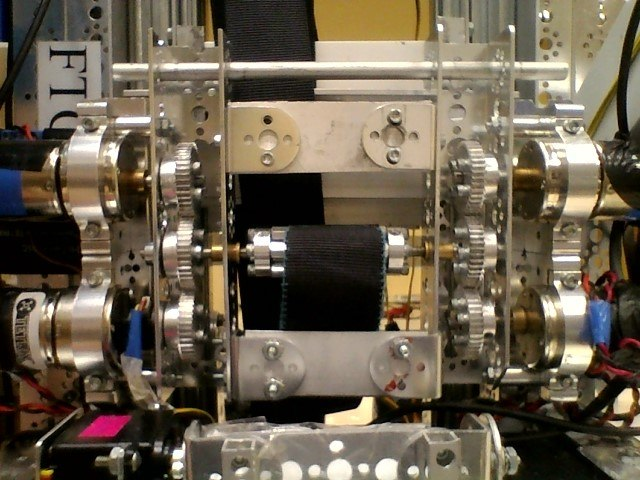
\includegraphics[scale=0.3]{days/29.11.14/images/01}}
				\caption{Измененный механизм лебедки}
			\end{minipage}
		\end{figure}
		
		\item Лебедка была испытана в действии. Скорость раздвигания подъемника увеличилась почти вдвое. В процессе раздвигания приводы подъемника не испытывали чрезмерных нагрузок. Мы остались удовлетворены работой механизма лебедки.
		
		\item Поскольку стяжки обладали недостаточной жесткостью и не всегда захватывали мячи, а также часто ломались, было решено использовать вместо них лопатки, вырезанные из цилиндрической части пластиковой бутылки. Было рассчитано, что наиболее оптимальное количество лопастей на оси захвата - 3. Кроме того, было решено усовершенствовать ковш, примыкающий к захвату, таким образом, чтобы с передней части он имел пандус высотой 7 см (размер большого шарика), на который лопатки захвата будут заталкивать мячи. Это позволит закидывать в ковш мячи в два яруса, что даст возможность захватить сразу пять больших мячей. Также эти мячи не будут вываливаться из ковша, поскольку им будет мешать пандус. Был создан схематичный чертеж захвата и ковша с пандусом.
		
		\begin{figure}[H]
			\begin{minipage}[h]{0.2\linewidth}
				\center  
			\end{minipage}
			\begin{minipage}[h]{0.6\linewidth}
				\center{
\includegraphics[scale=0.2]{days/29.11.14/images/02}}
				\caption{Схема взаимодействия захвата и ковша}
			\end{minipage}
		\end{figure}
		
	\end{enumerate}
	
	\item Итоги собрания: 
	\begin{enumerate}
		\item Механизм лебедки завершен. Теперь он приводится в движение не двумя, а четырьмя приводами.
		
		\item Лебедка испытана в действии. Скорость раздвигания подъемника увеличена почти вдвое.
		
		\item Конструкция нового механизма захвата мячей разработана.
		
	\end{enumerate}
	
	\item Задачи для последующих собраний:
	\begin{enumerate}
		\item Изменить механизм захвата мячей на более эффективный.
		
	\end{enumerate}     
\end{enumerate}
\fillpage